\documentclass{frontiersSCNS} 
\usepackage{url,hyperref,lineno,microtype,subcaption}
\usepackage[onehalfspacing]{setspace}
\linenumbers


\def\keyFont{\fontsize{8}{11}\helveticabold }
\def\firstAuthorLast{Marion {et~al.}} 
\def\Authors{Zachary H. Marion\,$^{1,*}$ and Christopher A. Hamm\,$^{2}$}
\def\Address{$^{1}$Department of Ecology \& Evolutionary Biology, University of Tennessee, Knoxville, TN, USA \\

$^{2}$Department of Ecology \& Evolutionary Biology, University of Kansas, Lawrence, KA, USA  }
\def\corrAuthor{Zachary H. Marion}
\def\corrEmail{zmarion@vols.utk.edu}

%%%%%%
%%%%%%
%%%%%%

\begin{document}
\onecolumn
\firstpage{1}

\title[Endosymbiont infection estimation]{A hierarchical Bayesian approach to estimate endosymbiont infection rates} 

\author[\firstAuthorLast ]{\Authors} %This field will be automatically populated
\address{} %This field will be automatically populated
\correspondance{} %This field will be automatically populated

\extraAuth{Department of Ecology \& Evolutionary Biology, University of Tennessee, 569 Dabney Hall, 1416 Circle Drive, Knoxville, TN, 37996, USA}

\maketitle
\begin{abstract}

\section{}
Endosymbionts may play an important role in the evolution of the Insecta. Bacteria such as \emph{Wolbachia, Cardinium, \emph{and} Rickettsia} are known to manipulate their host' reproduction to facilitate their own. Indeed, there are many well know cases where \emph{Wolbachia} (Alphaproteobacteria: Rickettsiaceae) induces one of four manipulative phenotypes (cytoplasmic incompatibility, male killing, feminization, and parthenogenesis). The scale of infection among species has been a major subject of investigation, but this is not an easy endeavor and different approaches have yielded different estimates. One aspect of this problem that may be underappreciated arises when multiple yet independent samples are taken within a species. When independent samples within species are treated as levels of a hierarchy the problem is greatly simplified because error propagates through the model in a realistic and intuitive manner. Here, we present a hierarchical Bayesian approach to estimate infection frequency where multiple independent samples were collected across multiple taxonomic levels. We apply this model to estimate the rates of infection for \emph{Wolbachia} in the Lepidoptera, and apply the model with a correction to account for phylogenetic non-independence. In addition, we highlight the present body of knowledge regarding \emph{Wolbachia} and its effects with regards to the Lepidoptera. Our model estimates suggests that the rate of endosymbiont infection in the Lepidoptera is lower than previously estimated. Given our limited knowledge regarding the phenotypes induced by these endosymbionts, we urge caution when interpreting the results of a positive assays.

\tiny
 \keyFont{ \section{Keywords:} \emph{Wolbachia}, Lepidoptera, modeling, butterfly, moth} % keywords should not be present in the title 
\end{abstract}

\section{Introduction}

Bacterial endosymbionts have been known to inhabit insects for decades. These endosymbionts are maternally transmitted through the cytoplasm of the egg. \textit{Wolbachia} was the first of these endosymbionts to be discovered when \citet{Hertig:1924wy} examined the adult ovaries and testes of \textit{Culex pipiens} (hence the specific epithet \textit{Wolbachia pipientis}) \citet{Hertig:1936}. Some years later, \citet{Yen:1971tc} observed that male \textit{C. pipiens} from one geographic area may not successfully reproduce with females from a different area, and reciprocal crosses could produce similar results; this phenomenon was given the name \textit{cytoplasmic incompatibility}. A \textit{Rickettsia}-like organism was determined to be the causative agent, which was later determined to be \textit{Wolbachia} \citep{Yen:1973vx}.

Contemporary researchers detect the presence of \textit{Wolbachia} via the polymerase chain reaction (PCR). Today, any sample can be screened in a quick, easy, and relatively inexpensive manner \citep{Baldo:2006p7025,Simoes:2011p11073}, however, this development is relatively recent. Prior to the advent of PCR, \textit{Wolbachia} infection was only confirmed through painstaking work that included electron microscopy and other microbiological techniques. Indeed, these methods required such effort that they were employed once a researcher had an \textit{a priori} reason suspect the presence of the bacterium; we are aware of no cases in which exploratory assays for \textit{Wolbachia} were conducted prior to the appearance of PCR. It was under these circumstances that a researcher would observe a likely reproductive manipulation phenotype (\emph{male killing, feminization, \emph{or} parthenogenesis}) and then attribute it to \textit{Wolbachia}.

Careful laboratory work is required to determine what phenotype (if any) is induced by an endosymbiont. With the arrival of PCR and Sanger sequencing it became feasible to conduct exploratory investigations for the presence of \textit{Wolbachia}, though few studies conducted the experimental work to determine if any reproductive manipulation was occurring. The effects of \textit{Wolbachia} infection are complex and depend on an interaction between the genomes of the endosymbiont and the host. For example, the phenotypic effects of one strain of \textit{Wolbachia} may be very different if moved into another host \citep{Rigaud:2001fv,Hoffmann:2011p11474}. Additionally, there may be extensive genomic differences between closely related strains of \textit{Wolbachia} \citep{Ishmael:2009p8257}. Though most famous for its status as a "reproductive parasite," \textit{Wolbachia} infections have been shown to induce no manipulation at all \citep{Hamm:2014cv,Zhang:2010jl,Zhang:2013eo}. Without careful experimentation, it is not scientific to assume that \textit{Wolbachia} will manipulate a host simply because of a positive PCR assay. 

The Lepidoptera (Arthropoda: Insecta) represent the best studied order of animals. Because of historic interest in their physical beauty and their contemporary economic importance the literature is replete with detailed knowledge regarding their distribution and life history. The  Lepidoptera is a large Order containing approximately 160,000 species in 124 families, which is approximately 13\% all species currently known \cite{Regier:2013fp}. In addition to research focused on the Lepidoptera for pure biological reasons, the Lepidoptera are also well represented on lists of endangered or threatened species \citep{Hamm:2014wi}. Researchers have tended to focus on certain groups of Lepidoptera, such as the butterflies (e.g. Nymphalidae, Lycaenidae and Pieridae) or groups of economically important pest species such as the Crambidae (which contains the Asiatic rice borer \textit{Chilo suppressalis} and Noctuidae (which contains the armyworms of the genus \textit{Spodoptera}); this results in a bias towards certain groups and leaves most of the remaining families understudied. 

Experiments to determine if a manipulative phenotype exits have been conducted for six species of Lepidoptera and report that \emph{cytoplasmic incompatibility, male killing, \emph{and} feminization} occur (Table 1). We note that the report of \textit{male killing} in \textit{Ephestia kuhniella} is a result of \textit{Wolbachia} transfected from \textit{Ostrinia scapulalis}. Because of the high level of interest in Lepidoptera research, there is a considered enthusiasm for investigating the role that \textit{Wolbachia} has played in its evolution. A vital first step towards this goal is the estimation of \textit{Wolbachia} infection rates in the Lepidoptera. 

ZACH, I'LL NEED TO YOU SET THE LAST PARAGRAPH OF THE INTRO. I CAN'T WRITE ABOUT IT WELL BUT MY ABORTED ATTEMPTS ARE BELOW.

Here, we develop and employ a novel approach to the estimation of \textit{Wolbachia} infection frequencies across the Lepidoptera. Our model explicitly accounts for issues that arise with real world data, such as those relating to estimating infection levels at different scales. For example, there may be multiple observations of infection frequency collected from different populations within a species, often with disparate sample sizes. We do not consider it appropriate for these samples to be completely pooled, as that ignores population differences in infection frequency. Nor should observations within species be considered independent, because of shared ancestry.  Similarly, there may be single samples collected from many different species within a family. In this case, individual sampling error should be accounted for when estimating family level infection rates. Finally, we consider that there has been a bias towards studying only a few families of the Lepidoptera. This uneven sampling can cause a few well-studied families to drive estimates of overall infection frequency. Each of these concerns can be specifically considered and accounted for with hierarchical Bayesian approaches that explicitly incorporate phylogenetic correlations. 


\section{Materials \& Methods}
\subsection{Motivating data and previous analyses}

 Both \cite{Weinert:2015aa} and \cite{Ahmed:2015aa} used a likelihood-based approach to describe the distribution of \emph{Wolbachia} infection across arthropods and Lepidoptera, respectively. Both studies used beta-binomial models to estimate the mean proportion of individuals infected within a given species \citep{Hilgenboecker:2008aa}. They used the same distribution to calculate the incidence of infection as well, where incidence was the proportion of species infected above a threshold frequency $c$  \citep[i.e.,, one infection in 1000 individuals, or 0.001;][]{Weinert:2015aa}. 

In the case of \textit{Wolbachia}, insects screened for this bacterium may either be positive or not positive. It is important to state that ?not positive? is the appropriate state here because an infection could have been missed for a number of reasons, including low density infections \citep{Schneider:2014jv}. However, for the sake of simplicity, we will treat \textit{Wolbachia} infection status as two mutually exclusive outcomes, (0 or 1; positive or not positive). This makes the question of infection a binomial sampling problem. The issue is the way that likelihood deals with error at each level, or rather how it does not. We will demonstrate this problem with two examples. First, let us assume that 200 individuals of a species are assayed for \textit{Wolbachia}, and 100 of those tests are positive for infection. The mean estimate of infection is 0.5 and the 95\% exact binomial confidence interval is 0.43 ? 0.57. Next, let us say that two individuals from a species were assayed for \textit{Wolbachia}, and one tested positive. For this example, the proportion infected in this species is 0.5, however, the 95\% confidence interval is 0.01 ? 0.99. It is clear that there is uncertainty around each estimate and that uncertainty varies with sample size. For this error to be properly incorporated into any estimate it must be treated at each level of the analysis (each species), rather than at the level of the study. 

\subsection{Data}
We used the data set synthesized by \citet{Weinert:2015aa}, which contains records from thousands of individual sampling efforts across the Arthropoda.  These data were arranged such that each row represented one independent sampling event (though each row may contain data from multiple individuals sampled) and contained information on the family, genus, species, endosymbiont genus, number of individuals assayed, and number of positive individuals. We filtered these data such that they contained only \textit{Wolbachia} assays of Lepidoptera. The filtered data set contained 1037 sampling events on 10860 individual Lepidoptera, of which 3607 screened positive for \textit{Wolbachia} infection. We imported these data into the program R v3.2 (R Core Development Team) and there conducted all subsequent analyses. All data and code necessary to reproduce the analyses and figures in this paper are freely available on FigShare (DOI TBD: \textit{NB}, the data will be accessioned to FigShare once the manuscript and code are in their final form).

To correct for any influence of the relatedness among families in our analysis, we used the Lepidoptera phylogeny of \citet{Regier:2013fp}, which contained 115 of the 124 families in the order. The tree was pruned to remove duplicate families and those not present in the  \cite{Weinert:2015aa} dataset. We then made the tree ultrametric following the penalized likelihood method of \citet{Sanderson:2002vy} using tools in the \textit{ape} package \citep{Paradis:2004dv}. To incorporate phylogenetic history into the Bayesian model, we used the pruned ultrametric tree to create a series of phylogenetic correlation matrices. We constructed one matrix in which we assumed that \textit{Wolbachia} infection status was distributed according to Brownian Motion (BM), a model of trait evolution that assumes neighboring taxa share that trait due to common ancestry \citep{Paradis:2012wn}. We also constructed matrices that assumed trait evolution followed an Ornstein-Uhlenbeck (OU) process, which places constraints around which a character evolves \citep{Paradis:2012wn}. Relative to the BM, the OU model has two additional parameters: $\theta$ (the "optimal" value for a character), and $\alpha$ (the rate at which $\theta$ moves towards $\alpha$) \citep{Paradis:2012wn}. The $\alpha$ value can range from 0 - 1; When $\alpha$ is 0 the model is effectively pure BM and becomes less so as $\alpha$ increases. We rescaled the Phylogeny using three alpha values to examine their impact: $\alpha$ = 0.1 (similar to BM), $\alpha$ = 0.5, and $\alpha$ = 0.9 (very different than BM).

\subsection{Bayesian hierarchical models}
	In contrast to \cite{Ahmed:2015aa}, we adopted a hierarchical Bayesian approach to estimate the probability of infection prevalence within and among species of Lepidoptera using a subset of the data from \cite{Weinert:2015aa}. Each observation ($N=1037$)---the number of \emph{Wolbachia}-infected individuals---was nested within species ($S=419$) and  modeled as:

\begin{equation}
	infected_{i,j} \sim \mathrm{Binomial}(n_{i}, \theta_{j}).
\end{equation}

where $i = 1, 2, \ldots, 1037$ and $j = 1, 2, \ldots, 419$. Here $infected_{i,j}$ indicates the number of infected individuals from the $i$th observation of the $j$th species,  $n_{i}$ is the total number of screened insects in observation $i$, and $\theta_{j}$ is the probability of infection for species $j$. 

	We then assumed the species-level probabilities of infection were normally-distributed with family-level means ($\mu_{k}$) and standard deviations ($\sigma_{k}$) where $k = 1, 2, \ldots, 28$ families. For computational efficiency, we used a non-centered parameterization of the normal \citep{Papaspiliopoulos:2007aa}. The normal distribution is unconstrained, but $\mathbf{\theta}$ is bounded between zero and one. Therefore the species-level $\theta$s were logit transformed such that  

	\begin{equation}    
		\mathrm{logit} (\theta_{j}) \sim \mathrm{Normal}(\mu_{k}, \sigma_{k}).
	\end{equation}
The mean ($\mu_{k}$) describes the average probability of infection within a lepidopteran species family on the log-odds scale and can be back-transformed using the inverse-logit function. 

The standard deviation ($\sigma$) measures how much variation in the probability of infection there is across species. If $\sigma$ is small, then infection probabilities will be similar among species. Conversely, if $\sigma$ is large, species-specific probabilities of infection will be more idiosyncratic. Data sparsity can be a problem in hierarchical models, especially for the estimation of scale parameters like variances. Because there were several species with few observations, we used a shrinkage prior \citep{Carvalho:2009aa,Carvalho:2010aa}
for the species-specific $\sigma$s: 
	\begin{align}
		\sigma_{k} 	&= 	 	t_{\nu}^{+}(0,\tau) \nonumber \\
        \tau		&\sim	t_{\nu}^{+}(0,1)     
	\end{align}

where $t_{3}^{+}$ is half-Student-t distribution with $\nu=3$ degrees of freedom. 

We modeled $\mu$, the vector of log-odds infection probabilities for families using a multivariate normal distribution:

\begin{equation}
	\begin{bmatrix}
		\mu_{1} \\
        \mu_{2} \\
        \vdots \\
        \mu_{k}
	\end{bmatrix}
    = 
    \textrm{MVNormal}(\gamma, \Sigma).
\end{equation}
with the mean log-odds probability of infection across Lepidoptera ($\gamma$) and covariance matrix $\Sigma$. To account for phylogenetic non-independence among families, we constructed sigma as:

\begin{equation}
	\Sigma = \boldsymbol{\eta} \;	\boldsymbol{\Omega} \; \boldsymbol{\eta}
\end{equation}

where $\boldsymbol{\eta}$ is a $k \times k$ diagonal matrix with the overall standard deviation on the diagonals and $\boldsymbol{\Omega}$ is a $k \times k$ phylogenetic correlation matrix. We then put regularizing priors on both $\gamma$ and $\eta$:

\begin{align}
	\gamma 	&\sim \mathrm{Normal}(0, 5) \nonumber \\
	\eta   	&\sim t_{\nu}^{+}(0,5)
\end{align}

where again $t_{3}^{+}$ is half-Student-t distribution with $\nu=3$ degrees of freedom. 

Posterior probabilities for model parameters were estimated using Markov chain Monte Carlo (MCMC) sampling in the Stan programming language \citep{Carpenter:2016aa} via the RStan interface \citep{stan:2016aa}. For each model, four MCMC chains were used with 5,000 iterations each. The first 2,500 iterations for each chain were adaptive and thus discarded as warm-up. We used several diagnostic tests to confirm that each model had reached a stationary distribution including visual examination of MCMC chain history and calculation of effective sample size (ESS) and the Gelman-Rubin convergence diagnostic \citep[$\hat{R}$; ][]{Gelman:1992aa,Brooks:1998aa}. In particular, model convergence was assessed by inspecting the diagnostics of the log-posterior density. Model fit was also assessed by posterior predictive checks by simulating ``new" data from the posterior distribution and plotting it against the original data. %Cite Gelman et al. 2013

We used WAIC \citep[the widely applicable or Watanabe-Akaike information criterion;][]{Watanabe:2010aa,Gelman:2014aa} to compare models with different phylogenetic correlation matrices (e.g., Brownian motion vs. OU processes) using functions in the loo package \citep{Vehtari:2016aa}. 

\section{Results}
After filtering the \citet{Weinert:2015aa} data to contain only Lepidoptera that were screened for \textit{Wolbachia} we retained 1037 independent sampling events with 411 unique species from 28 families, representing a total of 10860 individual assays. Of these, 3607 samples from 163 species and members of 19 families were scored PCR positive for \textit{Wolbachia}. 

The $\hat{R}$ diagnostic for all parameters (including the log-posterior density) was 1.0, indicating that each model had reached a stationary posterior distribution. Visual assessment of the MCMC chain history confirmed this. Additionally, the effective sample size for the log-posterior density was $> 2000$ for all models. Predictive plots of the posterior medians of the simulated ``new" observations regressed against the original observations resulted in tight concordance, suggesting the models were doing a good job at describing the data and providing a good fit. %make plots for supplement

All models, including those which contained phylogenetic correction, had similar WAIC scores with standard errors that completely overlapped (Table~\ref{aicTable}).  Therefore, each model was in the same ``family" of best models. Additionally, the results were almost identical across models, and all models predicted a median infection frequency of $\sim 15\%$. Rather than consider each model separately, we created a consensus model using model weighted averaging based on the $\Delta_{WAIC}$ scores (Table~\ref{aicTable}) to describe \emph{Wolbachia} infection frequency in the Lepidoptera. 

Our estimate for the median \emph{Wolbachia} infection frequency in the Lepidoptera was 12.1\% (95\% CI = 0.045 - 0.33; Figure~\ref{grand}) . Estimates for median family level infection frequency varied considerably with a positive association between sample size and credible interval (Figure~\ref{familyplot}). For example, the Lycaenidae (878 specimens from 346 species) and Nymphalidae (4060 specimens from 236 species) produced relatively tight distributions, while the families that had small sample sizes (e.g. Bombycidae, Hedylidae, and Lasiocampidae) generated larger credible intervals to reflect uncertainty in the estimates. 



\section{Discussion}
Our model predicts a median \emph{Wolbachia} infection rate for the Lepidoptera of approximately 12\%, an estimate that stands in considerable contrast to previously reported results. In a recent publication \citet{Ahmed:2015aa} estimated that approximately 80\% of lepidopteran species were infected at non-negligible frequencies. Similar to this estimate was that of \citet{Weinert:2015aa}, who reported \emph{Wolbachia} incidence rates of $\sim$75\% for the order Lepidoptera. Both of these studies employed similar approaches to estimate \emph{Wolbachia} infection rates, \citet{Ahmed:2015aa} employed a beta-binomial model  and \citet{Weinert:2015aa} employed both a beta and doubly-inflated beta, and also used very similar data sets. Employing the same data set as \citet{Weinert:2015aa} we arrived at a much lower estimate of \emph{Wolbachia} infection rate than either previous study examining the Lepidoptera. 

As with \citet{Weinert:2015aa}, we consider that there are three main sources of bias in the data set. From \citet{Weinert:2015aa} these biases are: 1\) some species are represented by a single sample, 2\) there is a taxonomic bias in the data, and 3\) research may be focused on groups with known \emph{Wolbachia} infection (e.g. \citet{Nice:2009p7399}). We also consider a fourth type of bias in the data, in that some families will be extensively sampled among a small number of different species, which may bias the data towards a few members of an otherwise large family of Lepidoptera.

We suggest that our infection rate estimate is lower than previous research because our hierarchical Bayesian model deals with these biases at each level and therefore may produce a more reliable estimate.

It is interesting to consider that our median infection frequency estimates for the Lepidoptera do not significantly change when the model considers relatedness by incorporating phylogenetic information (Figure~\ref{grand}). Additionally, the model WAIC scores were within 8 units of one another and their stand errors completely overlapped, implying that the models did not significantly vary among (Table~\ref{aicTable}). We interpret these results to indicate that our model is robust to differential sampling across the order Lepidoptera. We consider our estimate for median \emph{Wolbachia} infection rate for the Lepidoptera to be reliable and many of the family level estimates similarly so. We consider the family level estimates that are generated by large sample sizes to be reliable, but we must advise caution when interpreting some of these family level estimates when they are generated using small sample sizes. In these cases where one sample has been assayed for an entire family (Bombycidae, Callidulidae, Eupterotidae, Hedylidae, Lasiocampidae, Pterophoridae, Uraniidae) the estimates presented in Figure~\ref{familyplot} are driven by the grand mean for the Lepidoptera.

There are a number of interesting implications if our results accurately reflect the real prevalence of \emph{Wolbachia} in the Lepidoptera. If the infection frequency for species is on the order of 12\%, then perhaps \emph{Wolbachia} is not presently a major player in the evolution of this order.  It follows that, if \emph{Wolbachia} infection frequency is relatively low in the Lepidoptera than its role in the evolution of the order may not be as significant as with other groups \citep{Miller:2010ki}. Evidence is accumulating that demonstrates \emph{Wolbachia} is not an obligate manipulator or a host' reproductive biology \citep{Hamm:2014cv,Zhang:2010jl,Zhang:2013eo} and perhaps the paradigm needs to be reevaluated. Indeed, \citet{Prout:1994th} demonstrated that reproductive manipulator microbes should evolve to minimize harm to its host. 

The assumption that \emph{Wolbachia} always acts as a reproductive manipulator in incorrect \citep{Nice:2009p7399,Hamm:2014wi} and one must take significant care when extrapolating the results of a positive \emph{Wolbachia} assay into to real world effects. A \emph{Wolbachia} infection can impart benefits to its host, for example the \emph{wSuz} infection of \emph{Drosophila suzukii} confers resistance to certain viruses \citep{Cattel:IMB12245} and does not induce a manipulative phenotype \citep{Hamm:2014cv}. Thus, simply because \emph{Wolbachia} is detected does not and should not imply that the bacterium will be detrimental to its host. Furthermore, our knowledge of \emph{Wolbachia} as a reproductive manipulator in the Lepidoptera is based on scant evidence. To the best of our knowledge, of the 163 species of Lepidoptera considered positive for \emph{Wolbachia}, only seven species from four families have been assayed for an induced phenotype (Table~\ref{effects}). Reciprocal cross experiments are required to determine what (if any) effect \emph{Wolbachia} has on the reproduction of its host. Until these experiments are conducted for a particular system we urge extreme caution when interpreting a positive PCR assay and hope that researchers will conduct the necessary experiments to determine if a manipulative phenotype is even present in a particular system. 


In many respects, scientific research with regards to \textit{Wolbachia} is still in its "natural history" phase, wherein we describe the distribution and effects of infection.  
Need to conclude here, must think on it. 




\citet{vanNieukerken:2011a123}

\citet{Jiggins:2001p7754}

\citet{Jiggins:2001uo}


We conclude that the science of microbes in the Lepidoptera, especially with regards to the endosymbiont \textit{Wolbachia}, is still in its natural history phase wherein discovery is still largely in the descriptive phase, and as such we urge caution when interpreting positive \textit{Wolbachia} assays and extrapolating consequences. 



\newpage

%%%%%%
%%%%%%
%%%%%%

\section*{Conflict of Interest Statement}
The authors declare that the research was conducted in the absence of any commercial or financial relationships that could be construed as a potential conflict of interest.

%%%%%%
%%%%%%
%%%%%%

\section*{Author Contributions}
ZM and CH conceived of the experiment; ZM and CH conducted the analyses; ZM and CH wrote the manuscript. 

\section*{Funding}
The authors received no external funding to conduct this research.

\section*{Acknowledgments}
We wish to thank James Fordyce, Christopher Peterson, Brian O'Meara and Jeremy Beaulieu for their input and advice during the preparation of this manuscript. We also wish to thank Francis Jiggins and Jack Welch for discussions while this project was nascent. We also wish to thank the staff at the Tirimbina Biological Station for hosting us as we completed this manuscript. 

\section*{Supplemental Data}
 \href{http://home.frontiersin.org/about/author-guidelines#SupplementaryMaterial}{Supplementary Material} should be uploaded separately on submission, if there are Supplementary Figures, please include the caption in the same file as the figure. LaTeX Supplementary Material templates can be found in the Frontiers LaTeX folder 
\newpage
\bibliographystyle{frontiersinSCNS_ENG_HUMS} 
\bibliography{Wolbachia}
\newpage 

%%%%%%
%%%%%%
%%%%%%

\section*{Figures}

\begin{figure}[h!]
\begin{center}
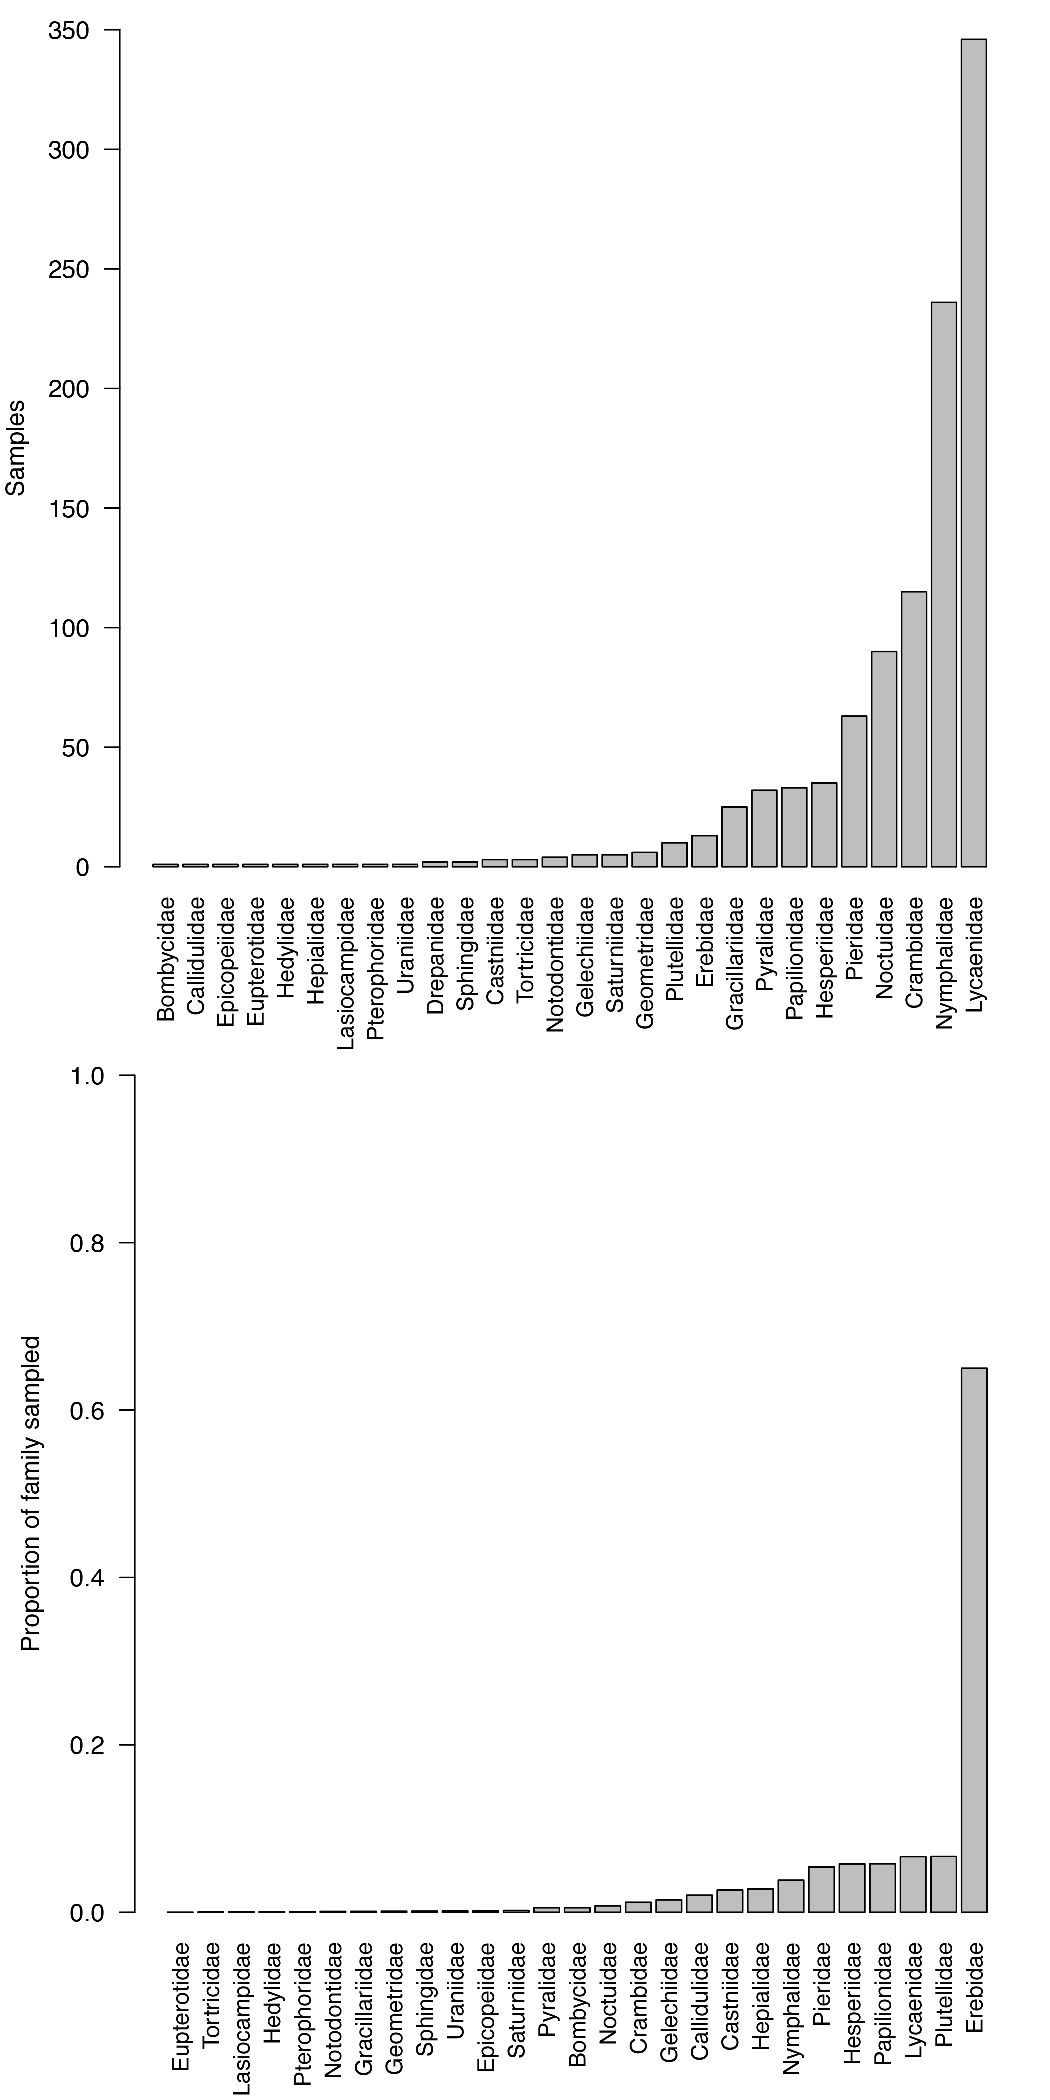
\includegraphics[width=85mm]{Fams_n_Props.pdf}% This is a *.jpg file
\end{center}
\caption{\textit{Wolbachia} sampling by family for total number \textbf{(A)} and scaled by proportion of species sampled in each family \textbf{(B)}.}
\label{histograms}
\end{figure}

\newpage

\begin{figure}[h!]
  \begin{center}
    \includegraphics[width=85mm]{infection_Prob.pdf}
    \caption{Posterior density plots for the average frequency of \textit{Wolbachia} infection across Lepidoptera. Each posterior estimate is jittered and superimposed on the violins with transparency. Fatter regions of the  violins indicate regions of higher posterior density, as do darker regions of jittered points. Horizontal bars indicate the median and upper and lower 95\% Highest Density Interval (HDI).  Models (L to R): NP = No Phylogenetic correction; BM = Brownian Motion; OU = Ornstein-Uhlenbeck with varying levels of $\alpha$ (0.1, 0.5, 0.9); Model Avg. = WAIC model weighted averaging.}
 \label{grand}
  \end{center}
\end{figure}

\newpage 

\begin{figure}[h!]
  \begin{center}
    \includegraphics[width=180mm]{familyplotAvg.pdf}
    \caption{Posterior density plots for the average frequency of \textit{Wolbachia} infection among 28 families of Lepidoptera. Each posterior estimate is jittered and superimposed on the violins with transparency. Fatter regions of the  violins indicate regions of higher posterior density, as do darker regions of jittered points. Horizontal bars indicate the median and upper and lower 95\% Highest Density Interval (HDI).}
 \label{familyplot}
  \end{center}
\end{figure}
\newpage

%%%%%%
%%%%%%
%%%%%%

\section*{Tables}



\begin{table}[h!] \centering 
  \caption{Models with different phylogenetic correlation structures ranked according to WAIC and their respective model weights. The no-phylogeny model had an identity matrix (ones on the diagonal and zeros on the off-diagonals) in place of a correlation matrix. Smaller WAIC values indicate better estimates. $\Delta_{\mathrm{waic}}$ is the difference between each WAIC and the lowest WAIC value. SE$_{\mathrm{waic}}$ and SE$_\Delta$ are the standard errors for WAIC and $\Delta_{\mathrm{waic}}$ respectively.}
  
  \label{aicTable} 
\begin{tabular}{@{\extracolsep{5pt}} lcccccc} 
\\
\\[-1.8ex]\hline 
\hline \\[-1.8ex] 
Model & WAIC & SE$_{\mathrm{waic}}$ & $p_{\mathrm{waic}}$ & $\Delta_{\mathrm{waic}}$ & SE$_\Delta$ & weight \\ 
\hline \\[-1.8ex] 
OU: $\alpha=0.1$ & $3,458.7$ & $318.1$ & $245.2$ & $0.0$ & $ $ & $0.79$ \\ 
OU: $\alpha=0.5$ & $3,462.8$ & $319.7$ & $245.7$ & $4.1$ & $2.55$ & $0.10$ \\ 
Brownian Motion & $3,464.1$ & $320.3$ & $246.6$ & $5.4$ & $3.44$ & $0.05$ \\ 
No Phylogeny & $3,464.9$ & $320.2$ & $247.9$ & $6.3$ & $3.07$ & $0.03$ \\ 
OU: $\alpha=0.9$ & $3,465.9$ & $320.1$ & $247.1$ & $7.2$ & $3.13$ & $0.02$ \\ 




\hline \\[-1.8ex] 
\\
\end{tabular} 
\end{table} 




\begin{table}[h!] \centering
  \caption{Published phenotypic effects of \textit{Wolbachia} on Lepidoptera.  Phenotype: MK = male killing, Fem = feminization, CI = cytoplasmic incompatibility. * = induced by transfection with \textit{Wolbachia} strain from \textit{O. scapulalis}.} 
  
  \label{effects}
\begin{tabular}{@{\extracolsep{5pt}} l c c c}
\\
\\[-1.8ex]\hline 
Species & Family & Phenotype & Reference\\
\hline \\[-1.8ex] 
\textit{Acrea encedana}& Nymphalidae & MK & \citet{Jiggins:2000gz}\\
\textit{Acraea encedon} & Nymphalidae & MK & \citet{Jiggins:1998p7753}\\
\textit{Ephestia kuehniella}* & Pyralidae & MK & \citet{Fujii:2001p8208}\\
\textit{Eurema hecabe} & Pieridae & CI & \citet{Narita:2007p8218}\\
\textit{Hypolimnas bolima} & Nymphalidae & MK & \citet{Dyson:2002p8665,Mitsuhashi:2004p8229}\\
\textit{Ostrinia scapulalis} & Crambidae & MK \& Fem & \citet{Sugimoto:2012ge}\\
\textit{Ostrinia furnacalis} & Crambidae & Fem & \citet{Kageyama:2002p8664}\\
\hline \\[-1.8ex] 
\\
\end{tabular}
\end{table}


\end{document}
